\documentclass[letter,12pt]{article}


\usepackage[english]{babel}

\usepackage{fancyhdr}


\usepackage{graphicx}
\usepackage{amsmath}
\usepackage{amssymb}
\usepackage[latin1]{inputenc}
\usepackage{fancybox}
\usepackage{amsfonts}
\usepackage{bbold}
\usepackage{textcomp}

\usepackage{subcaption}
\usepackage{booktabs, array, dcolumn}
\newcommand{\ra}[1]{\renewcommand{\arraystretch}{#1}}
\newcolumntype{d}{D{.}{.}{2.3}}
\newcolumntype{C}{p}


\setlength{\oddsidemargin}{0in}
\setlength{\evensidemargin}{0in}
\setlength{\textwidth}{16.1 cm}
\setlength{\topmargin}{-15mm}
\setlength{\textheight}{22cm}
\setlength{\parindent}{0cm}



%% calligraphic
\newcommand{\cA}{{\cal A}}
\newcommand{\cB}{{\cal B}}
\newcommand{\cC}{{\cal C}}
\newcommand{\cD}{{\cal D}}
\newcommand{\cF}{{\cal F}}
\newcommand{\cG}{{\cal G}}
\newcommand{\cI}{{\cal I}}
\newcommand{\cL}{{\cal L}}
\newcommand{\cM}{{\cal M}}
\newcommand{\cN}{{\cal N}}
\newcommand{\cO}{{\cal O}}
\newcommand{\cP}{{\cal P}}
\newcommand{\cR}{{\cal R}}
\newcommand{\cW}{{\cal W}}
%% calligraphic composite
\newcommand{\cMA}{{\cal MA}}
\newcommand{\cMU}{{\cal MU}}


%% double line letters
\newcommand{\rA}{\mathbb{A}}
\newcommand{\rB}{\mathbb{B}}
\newcommand{\rC}{\mathbb{C}}
\newcommand{\rF}{\mathbb{F}}
\newcommand{\rK}{\mathbb{K}}
\newcommand{\rR}{\mathbb{R}}
\newcommand{\rS}{\mathbb{S}}
\newcommand{\rSp}{\mathbb{S}^{\prime}}
\newcommand{\rP}{\mathbb{P}}
\newcommand{\rU}{\mathbb{U}}
\newcommand{\rV}{\mathbb{V}}
\newcommand{\rW}{\mathbb{W}}
\newcommand{\rZ}{\mathbb{Z}}



%% bold
\newcommand{\bfm}[1]{\mathbf{#1}}
\newcommand{\bsn}[1]{\boldsymbol{#1}}


%% upright
\newcommand{\txtg}{\text{g}}
\newcommand{\txtu}{\text{u}}
\newcommand{\txte}{\text{e}}
\newcommand{\txtv}{\text{v}}
\newcommand{\txta}{\text{a}}
\newcommand{\txtb}{\text{b}}
\newcommand{\txtT}{\text{T}}

%% underline
\newcommand{\uun}[1]{\underline{\underline{#1}}}
\newcommand{\un}[1]{\underline{#1}}
%\newcommand{\Gradu}{\underline{\nabla}}
%\newcommand{\Graduu}{\underline{\underline{\nabla}}}
%\newcommand{\gradu}{\underline{\text{grad}}}
%\newcommand{\graduu}{\underline{\underline{\text{grad}}}}
%\newcommand{\graduu}{\underline{\underline{\underline{\text{grad}}}}}
\newcommand{\Grad}{\nabla}
\newcommand{\Gradu}{\underline{\nabla}}
\newcommand{\Graduu}{\underline{\underline{\nabla}}}
\newcommand{\grad}{\text{grad}}
\newcommand{\gradu}{\text{grad}}
\newcommand{\graduu}{\text{grad}}
\newcommand{\graduuu}{\text{grad}}
\newcommand{\rot}{\text{curl}}
\newcommand{\rotu}{\text{curl}}
\newcommand{\zerou}{\underline{0}}
%% double underline
\newcommand{\tm}{\uun{\tt{1}\!\!\tt{l}}}    %
\newcommand{\zerouu}{\underline{\underline{0}}}
%% underline italic
\newcommand{\au}{\underline{a}}
\newcommand{\Au}{\underline{A}}
\newcommand{\bu}{\underline{b}}
\newcommand{\Bu}{\underline{B}}
\newcommand{\Cu}{\underline{C}}
\newcommand{\cu}{\underline{c}}
\newcommand{\eu}{\underline{e}}
\newcommand{\fu}{\underline{f}}
\newcommand{\Fu}{\underline{F}}
\newcommand{\gu}{\underline{g}}
\newcommand{\txtgu}{\underline{\txtg}}
\newcommand{\Gu}{\underline{G}}
\newcommand{\Mu}{\underline{M}}
\newcommand{\iu}{\underline{i}}
\newcommand{\ku}{\underline{k}}
\newcommand{\nnu}{\underline{n}}
\newcommand{\Nu}{\underline{N}}
\newcommand{\pu}{\underline{p}}
\newcommand{\Pu}{\underline{P}}
\newcommand{\qu}{\underline{q}}
\newcommand{\Qu}{\underline{Q}}
\newcommand{\Ru}{\underline{R}}
\newcommand{\ru}{\underline{r}}
\newcommand{\su}{\underline{s}}
\newcommand{\tu}{\underline{t}}
\newcommand{\Tu}{\underline{T}}
\newcommand{\uu}{\underline{u}}
\newcommand{\Uu}{\underline{U}}
\newcommand{\vu}{\underline{v}}
\newcommand{\Vu}{\underline{V}}
\newcommand{\wu}{\underline{w}}
\newcommand{\xu}{\underline{x}}
\newcommand{\Xu}{\underline{X}}
%% double underline italic
\newcommand{\Auu}{\underline{\underline{A}}}
\newcommand{\Buu}{\underline{\underline{B}}}
\newcommand{\Cuu}{\underline{\underline{C}}}
\newcommand{\Duu}{\underline{\underline{D}}}
\newcommand{\Euu}{\underline{\underline{E}}}
\newcommand{\duu}{\underline{\underline{d}}}
\newcommand{\hduu}{\hat{\duu}}
\newcommand{\euu}{\underline{\underline{e}}}
\newcommand{\Fuu}{\underline{\underline{F}}}
\newcommand{\fuu}{\underline{\underline{f}}}
\newcommand{\Guu}{\underline{\underline{G}}}
\newcommand{\Huu}{\underline{\underline{H}}}
\newcommand{\Iuu}{\underline{\underline{I}}}
\newcommand{\kuu}{\underline{\underline{k}}}
\newcommand{\Kuu}{\underline{\underline{K}}}
\newcommand{\Puu}{\underline{\underline{P}}}
\newcommand{\Quu}{\underline{\underline{Q}}}
\newcommand{\Ruu}{\underline{\underline{R}}}
\newcommand{\Suu}{\underline{\underline{S}}}
\newcommand{\Tuu}{\underline{\underline{T}}}
\newcommand{\Uuu}{\underline{\underline{U}}}
\newcommand{\hUuu}{\hat{\Uu}}
\newcommand{\wuu}{\underline{\underline{w}}}
%% underline greco
\newcommand{\alphau}{\underline{\alpha}}
\newcommand{\tauu}{\underline{\tau}}
\newcommand{\deltau}{\underline{\delta}}
\newcommand{\Gammau}{\underline{\Gamma}}
\newcommand{\chiu}{\underline{\chi}}
\newcommand{\piuu}{\underline{\underline{S}}}
\newcommand{\Omu}{\underline{\Omega}}
\newcommand{\Omegau}{\underline{\Omega}}
\newcommand{\hOmegau}{\hat{\Omegau}}
\newcommand{\omegau}{\underline{\omega}}
\newcommand{\lambdau}{\underline{\lambda}}
\newcommand{\phiu}{\underline{\phi}}
\newcommand{\varphiu}{\underline{\varphi}}
\newcommand{\psiu}{\underline{\psi}}
\newcommand{\xiu}{\underline{\xi}}
%% double underline greek
\newcommand{\alphauu}{\underline{\underline{\alpha}}}
\newcommand{\betauu}{\underline{\underline{\beta}}}
\newcommand{\epsuu}{\underline{\underline{\varepsilon}}}
\newcommand{\vepsuu}{\underline{\underline{\varepsilon}}}
\newcommand{\Omuu}{\underline{\underline{\Omega}}}
\newcommand{\Omegauu}{\underline{\underline{\Omega}}}
\newcommand{\sigmauu}{\underline{\underline{\sigma}}}
\newcommand{\Sigmauu}{\underline{\underline{\Sigma}}}

%% primes
\newcommand{\Op}{O^{\prime}}
\newcommand{\Sigmap}{\Sigma^{\prime}}
\newcommand{\eup}{\eu^{\prime}}


%% measures italic
\newcommand{\da}{{\text d}a}
\newcommand{\dA}{{\text d}A}
\newcommand{\dell}{{\text d}\ell}
\newcommand{\dr}{{\text d}r}
\newcommand{\dR}{{\text d}R}
\newcommand{\dS}{{\text d}S}
\newcommand{\ds}{{\text d}s}
\newcommand{\dt}{{\text d}t}
\newcommand{\dx}{{\text d}x}
\newcommand{\dy}{{\text d}y}
\newcommand{\dz}{{\text d}z}
\newcommand{\dV}{{\text d}V}
\newcommand{\dX}{{\text d}X}
\newcommand{\dY}{{\text d}Y}
\newcommand{\dZ}{{\text d}Z}
%% measures greek
\newcommand{\dphi}{{\text d}\phi}
\newcommand{\dOmega}{{\text d}\Omega}
\newcommand{\dtheta}{{\text d}\theta}
\newcommand{\dlambda}{{\text d}\lambda}
%% measures undelined
\newcommand{\dau}{\underline{\da}}
\newcommand{\dAu}{\underline{\dA}}
\newcommand{\dlu}{{\text d}\ell}
\newcommand{\dMu}{\underline{{\text d}M}}
\newcommand{\dUu}{\underline{{\text d}U}}
\newcommand{\dxu}{\underline{{\text d}x}}
\newcommand{\dXu}{\underline{{\text d}X}}


%% hat and dots
\newcommand{\hU}{\hat{U}}
\newcommand{\hUu}{\hat{\Uu}}
\newcommand{\hd}{\hat{d}}
\newcommand{\hq}{\hat{q}}
\newcommand{\hu}{\hat{u}}
\newcommand{\hdot}[1]{\hat{\dot{#1}}}
\newcommand{\hdtheta}{\hat{\dot{\theta}}}
\newcommand{\hepsilon}{\hat{\varepsilon}}
\newcommand{\hxi}{\hat{\xi}}
\newcommand{\hsigma}{\hat{\sigma}}
\newcommand{\homega}{\hat{\omega}}
\newcommand{\hxiu}{\hat{\xiu}}



%% derivatives
\newcommand{\dert}[2]{\frac{\text{d}#1}{\text{d}#2}}
\newcommand{\derp}[2]{\frac{\partial #1}{\partial #2}}
\newcommand{\der}[2]{\frac{\partial #1}{\partial #2}}
\newcommand{\derpd}[2]{\frac{\partial^{2}#1}{\partial#2^{2}}}
\newcommand{\derpc}[3]{\frac{\partial^{2}#1}{\partial#2 \partial#3}}
\newcommand{\linederp}[2]{(\partial#1/\partial#2)}


%% sinalpha cosalpha
\newcommand{\sina}{\sin\!\alpha}
\newcommand{\sinad}{\sin^2\!\alpha}
\newcommand{\cosa}{\cos\!\alpha}
\newcommand{\cosad}{\cos^2\!\alpha}
\newcommand{\cosda}{\cos\! 2\alpha}
\newcommand{\sinda}{\sin\! 2\alpha}
\newcommand{\cota}{\cot\!\alpha}
\newcommand{\cotad}{\cot^2\!\alpha}

%% sinteta costeta
\newcommand{\sinteta}{\sin\!\theta}
\newcommand{\sintetad}{\sin^2\!\theta}
\newcommand{\costeta}{\cos\!\theta}
\newcommand{\costetad}{\cos^2\!\theta}
\newcommand{\cosdteta}{\cos\! 2\theta}
\newcommand{\sindteta}{\sin\! 2\theta}
\newcommand{\cotteta}{\cot\!\theta}
\newcommand{\cottetad}{\cot^2\!\theta}


%% tenseur cilyndiques et spheriques
\newcommand{\sigmatt}{\sigma_{\vartheta\vartheta}}
\newcommand{\sigmarr}{\sigma_{rr}}
\newcommand{\sigmart}{\sigma_{r\vartheta}}
\newcommand{\sigmatr}{\sigma_{\vartheta r}}
\newcommand{\sigmatz}{\sigma_{\vartheta z}}
\newcommand{\sigmazt}{\sigma_{z\vartheta}}
\newcommand{\sigmazz}{\sigma_{zz}}
\newcommand{\sigmarz}{\sigma_{rz}}
\newcommand{\sigmazr}{\sigma_{zr}}
\newcommand{\sigmaff}{\sigma_{\varphi\varphi}}
\newcommand{\epstt}{\varepsilon_{\vartheta\vartheta}}
\newcommand{\epsrr}{\varepsilon_{rr}}
\newcommand{\epsrt}{\varepsilon_{r\vartheta}}
\newcommand{\epstr}{\varepsilon_{\vartheta r}}
\newcommand{\epsrz}{\varepsilon_{rz}}
\newcommand{\epszr}{\varepsilon_{zr}}
\newcommand{\epstz}{\varepsilon_{\vartheta z}}
\newcommand{\epszt}{\varepsilon_{z\vartheta}}
\newcommand{\epszz}{\varepsilon_{zz}}
\newcommand{\epsff}{\varepsilon_{\varphi\varphi}}


%% ref. spaces
\newcommand{\rf}[1]{eqn.~(\ref{#1})}
\newcommand{\rfs}[2]{eqns.~(\ref{#1}) and (\ref{#2})}
\newcommand{\hs}[1]{\hspace{#1cm}}
\newcommand{\vs}[1]{\vspace{#1cm}}
\newcommand{\hhs}[1]{\hspace*{#1cm}}
\newcommand{\vvs}[1]{\vspace*{#1cm}}
\newcommand{\pre}[3]{\vspace{-.6\baselineskip}\bibitem{#3}}
\newcommand{\nnum}{\nonumber \\[1ex]}
\newcommand{\stext}[1]{\quad\text{#1}\quad}
\newcommand{\sstext}[1]{\qquad\text{#1}\qquad}


%% miscellanea
\newcommand{\Psip}{\Psi^{\prime}}
\newcommand{\eps}{\varepsilon}
\newcommand{\defi}{\overset{\text{def}}{=}}
\newcommand{\diad}[2]{\eu_{#1}\otimes\eu_{#2}}
\newcommand{\tr}{\text{tr}}    %
\newcommand{\diver}{\text{div}}    %
\newcommand{\diverp}{\text{div}^{\prime}}    %
\newcommand{\DIV}{\text{DIV}}    %
\newcommand{\tran}{\,^{t}}
\newcommand{\nsum}[1]{\quad\text{sans sommation sur}\quad #1}
\renewcommand{\baselinestretch}{1.}
\newcommand{\abs}[1]{\left| #1 \right|}
\newcommand{\inv}[1]{I^{\prime}_{#1}}    %
\newcommand{\ppl}{[\![}    %
\newcommand{\ppr}{]\!]}    %
\newcommand{\p}{^\prime}    %
\newcommand{\pp}{^{\prime\prime}}    %
\newcommand{\ruun}[1]{\underline{\underline{\mathrm{#1}}}}
\newcommand{\run}[1]{\underline{\mathrm{#1}}}
\newcommand{\tel}{\text{el}}
\renewcommand{\vec}[1]{\left\{#1\right\}}
\newcommand{\mat}[1]{\left[#1\right]}

\newcommand{\opic}{o\left(\|\nabla\xiu\|\right)}
\newcommand{\vphil}{\phi}

\usepackage{alltt}
\usepackage{boxedminipage}
\usepackage{float}
\newenvironment{code}{
\footnotesize
\begin{alltt}
\begin{center}
%\begin{boxedminipage}{1.0\textwidth}
\begin{minipage}{1.0\textwidth}
}{
\end{minipage}
%\end{boxedminipage}
\end{center}
\end{alltt}
}

\newtheorem{teorem}{Th�or�me}

%%%%%%%%%%%%%%%%%%%%%%%%%%%%%%%%%%%%%%%%%%%%%%%%%%%%%%%
\makeatletter
\newcommand{\risposta}{\@startsection
{risposta}%
{2}%
{0mm}%
{-\baselineskip}%
{.5\baselineskip}%
{\normalfont\normalsize\bfseries\itshape}}%
\makeatother

%definition of list of items
\newcommand{\entrylabel}[1]{\mbox{\textsf{#1:}}\hfil}
\newenvironment{entry}
 {\begin{list}{}%
   {\renewcommand{\makelabel}{\entrylabel}%
     \setlength{\labelwidth}{3cm}%
     \setlength{\leftmargin}{\labelwidth+\labelsep}%
   }%
 }%
 {\end{list}}

\newenvironment{Ventry}[1]%
 {\begin{list}{}{\renewcommand{\makelabel}[1]{\bfseries\textsf{##1:}\hfil}%
   \settowidth{\labelwidth}{\textsf{#1:}}%
   \setlength{\leftmargin}{\labelwidth+\labelsep}}}%
 {\end{list}}


%%%%%%%%%%%%%%%%%%%%%%%%%%%%%%%%%%%%%%%%%%%%%%%%%%%%%%%

\newcounter{risposta}[section]
\renewcommand{\therisposta}{Point \arabic{risposta}}
\newcommand{\D}{\displaystyle}

\newcommand{\sv}{\underline}
\newcommand{\Sig}{\boldsymbol{\sigma}}
\newcommand{\K}{\boldsymbol{K}}
\newcommand{\Eps}{\boldsymbol{\varepsilon}}
\newcommand{\intener}{\mathcal{E}}


% --------------------------------------------------------------------------------------
% - definition des notations
% --------------------------------------------------------------------------------------




\begin{document}
\pagestyle{fancy}

\title{\textbf{Practice: \\ Static and Kinematic Admissibility}}
\date{}

\maketitle

\vspace{-1cm}


%\section{Problem 1 }
%A homogeneous continuum as in Fig. 1 is clamped on surface $S_3^-(z = 0)$  and submitted to a uniform pressure $p_0$ over the surface $S_1^+(x=l_1)$. \\
%%
%
%\noindent \textbf{Question 1}: Write the static admissibility equations! \\
%
%\noindent \textbf{Question 2}: Write the kinematic admissibility equations! \\
%
%\noindent \textbf{Question 3}: Assuming we use the Cartesian coordinate system, please give the expansion of these equations! \\
%
%\noindent \textbf{Question 4}: Calculate $\int_{S_3^-} \sigmauu \cdot \underline{n}  \quad dS$ \\



\section*{Problem 2}
Let us consider a sphere with cavity (exterior radius $R_e$ and internal radius $R_i$). The external surface $S_e$ is free of loading and the interior surface $S_i$ is submitted to a pressure $p_0$. The material is assumed to be isotropic linear elastic with young modulus $E$ and Poisson ratio $\nu$. \\

\begin{figure}[ht]
	\centering
	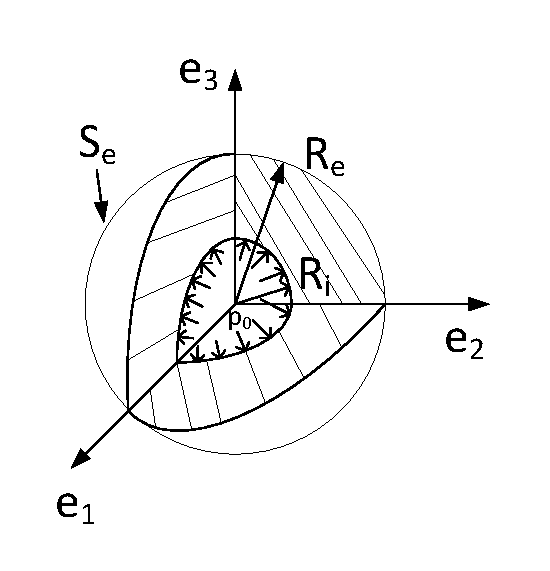
\includegraphics[width=0.5\textwidth]{figures/p2}
	\caption{Configuration of problem 2}
	\label{fig:problem2}
\end{figure}


\noindent \textbf{Question 1}: Write the static admissibility equations! \\

\textbf{Answer:} Find $\sigmauu $ symmetric such that 
\begin{equation}
\begin{split}
& \text{(a)  } \sigmauu \cdot \underline{n} = \underline{0} \quad \forall \text{ } M \in S_e \quad \text{Boundary equation} \\
& \text{(b)  } \sigmauu \cdot \underline{n} = - p_0 \underline{n} \quad \forall \text{ } M \in S_i \quad \text{Boundary equation} \\
& \text{(c)  } \divu \sigmauu = \underline{0} \quad \forall \text{ } M \in \Omega \quad \text{Internal equilibrium}
\end{split}
\end{equation}

\noindent \textbf{Question 2}: Please expand this equation using spherical  coordinates system! \\

\textbf{Answer:} In spherical coordinates,
\begin{equation}
\sigmauu = \left[
\begin{matrix}
\sigmarr & \sigmart & \sigmarf \\
\sigmart & \sigmatt & \sigmatf \\
\sigmarf & \sigmatf & \sigmaff 
\end{matrix}
\right]
\end{equation}

From Eq. (a),
\begin{equation}
\sigmarr(r = R_e,\theta,\varphi) = \sigmart (r=R_e,\theta,\varphi) = \sigmarf(r=R_e,\theta,\varphi) = 0
\end{equation}

From Eq. (b),
\begin{equation}
\begin{split}
& -\sigmarr(r=R_i,\theta,\varphi) = p_0 \\
& -\sigmart(r=R_i,\theta,\varphi) = 0 \\
& -\sigmarf(r=R_i,\theta,\varphi) = 0
\end{split}
\end{equation}

From Eq. (c) $\rightarrow$ See Textbook equation 1.11a (divergence with spherical coordinates)



\noindent \textbf{Question 3}: Let's assume that the following stress tensor 
\begin{equation}
\sigmauu = \left[ \begin{matrix}
\sigmarr &0 &0 \\
0 & \sigmatt & 0 \\
0 & 0 & \sigmaff
\end{matrix} \right]
\end{equation}
with 
\begin{equation}
\sigmarr = -A\left[\frac{B}{r^3} - 1 \right]
\end{equation}
and 
\begin{equation}
\sigmatt = \sigmaff = A \left[\frac{B}{2r^3} + 1 \right]
\end{equation}
Please calculate the coefficient $A$ and $B$ so that $\sigmauu$ could be a solution of the problem! \\ 

\textbf{Answer:} Using the proposed stress tensor, and expanding equation (c), we get
\begin{equation}
\begin{split}
& \derp{\sigmarr}{r} + \frac{2\sigmarr - \sigmatt - \sigmaff}{r} = 0 \\
& 0 = 0 \\
& 0 = 0
\end{split}
\end{equation}
We now check if $\sigmauu$ ca fulfill the static admissibility equations.
\begin{equation}
\derp{\sigmarr}{r} + \frac{2\sigmarr - \sigmatt - \sigmaff}{r} = \frac{3AB}{r^4} - \frac{3AB}{r^4} = 0 \rightarrow \text{(c) is OK. Interior equilibrium is satisfied.}
\end{equation}
\begin{equation}
\text{(a)} \rightarrow - A\left[
\frac{B}{R_e^3} - 1 \right] = 0 \rightarrow B = R_e^3
\end{equation}

\begin{equation}
\text{(b)} \rightarrow - A\left[
\frac{R_i^3}{R_e^3} - 1 \right] = p_0 \rightarrow A = p_0 \frac{R_e^3}{R_i^3 - R_e^3}
\end{equation}\\

All the other conditions concerning $\sigmatr$ and $\sigmarf$ are automatically satisfied due to the chosen stress tensor. Thus, a statically admissible stress field is:
\begin{equation}
\sigmauu = \left[
\begin{matrix}
p_0 \frac{R_e^3}{R_i^3 - R_e^3} \left[
\frac{R_i^3}{r} - 1 \right] & 0 & 0 \\
0 & -p_0 \frac{R_e^3}{R_e^3 - R_i^3} \left[
\frac{R_e^3}{2r^3} + 1 \right] & 0 \\
0 & 0 & -p_0 \frac{R_e^3}{R_e^3 - R_i^3} \left[
\frac{R_e^3}{2r^3} + 1 \right]
\end{matrix}
\right]
\end{equation} \\



\noindent \textbf{Question 4}: Please calculate the strain tensor $\epsuu$? Does it satisfy the compatibility equation? Conclusion?

\textbf{Answer:} Based on the constitutive equation, we can calculate the strains:
\begin{equation}
\epsuu = \frac{1+\nu}{E} \sigmauu - \frac{\nu}{E} \text{tr} \sigmauu \underline{\underline{1}}
\end{equation}
\begin{equation}
\text{tr}\sigmauu = -p_0 \frac{R_e^3}{R_e^3 - R_i^3}
\end{equation}
Thus, we get $\epsrt = \epstf = \epsft = 0$. Let us note that 
\begin{equation}
A_1 = p_0 \frac{R_e^3}{R_e^3 - R_i^3}
\end{equation}

We get:
\begin{equation}
\epsuu =  \left[
\begin{matrix}
\left(\frac{1+\nu}{E}\right) A_1 \left[
\frac{R_e^3}{r} - 1 \right] + \frac{\nu}{E} A_1 & 0 & 0 \\
0 & -\left(\frac{1+\nu}{E}\right) A_1 \left[
\frac{R_e^3}{2r^3} + 1 \right] + \frac{\nu}{E} A_1 & 0 \\
0 & 0 & -\left(\frac{1+\nu}{E}\right) A_1 \left[
\frac{R_e^3}{2r^3} + 1 \right] + \frac{\nu}{E} A_1
\end{matrix}
\right]
\end{equation} \\

In case of complete spherical symmetry, the compatibility equation can be simplified (see Textbook equation 2.14b):
\begin{equation}
\frac{d\epsff}{dr} + \frac{\epsff- \epsrr}{r} = 0
\end{equation}
Let us verify if this equation is satisfied by $\epsuu$.
\begin{equation}
\frac{d\epsff}{dr} = 3A_1 \left(\frac{1+\nu}{E}\right) \frac{R_e^3}{2r^4}
\end{equation}
\begin{equation}
\frac{\epsff - \epsrr}{r} = -3A_1 \left(\frac{1+\nu}{E}\right) \frac{R_e^3}{2r^4}
\end{equation} \\

The two equations above satisfied the compatibility equation. Thus it will be possible to integrate $\epsuu$ to determine a displacement field $\underline{u}$. Considering there is no additional kinematic condition (no kinematic boundary condition), we got the exact solution of the problem.





\newpage
\section*{Problem 3}
Let us consider a domain $\Omega$, simply supported by a rigid basis ($\Gamma$). $\Omega$ is submitted to gravity volume forces $\fu = \rho g \underline{y} $ and to uniform pressure $p > 0$ over every vertical side. We assume plane stresses in the plane of $x-y$ and the material is isotropic linear elastic with Young modulus $E$ and Poisson ratio $\nu$. \\

\begin{figure}[ht]
	\centering
	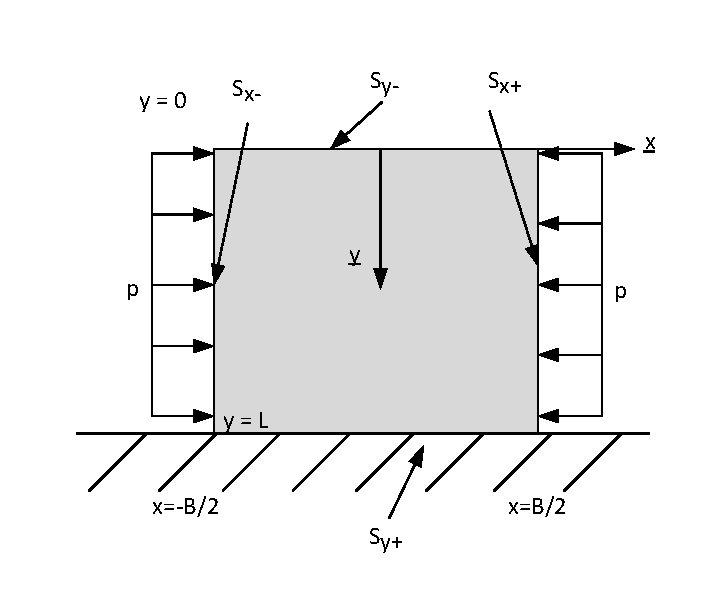
\includegraphics[width=0.6\textwidth]{figures/p3}
	\caption{Configuration of problem 3}
	\label{fig:problem3}
\end{figure}

\noindent \textbf{Question 1}: Write down the full problem! (kinematic, static and constitutive equations) \\

\textbf{Answer:} 
\textbf{Kinematic admissibility:}\\
Let us not $\uu$ the displacement vector such that $\uu=\left(\begin{matrix}
u \\ v
\end{matrix} \right) $, $\uu=u\xu+v \underline{y}$\\
\begin{equation}
\left\lbrace \begin{matrix}
v=0, \quad \forall M \in S_y^+ \\
\underline{\underline{\epsilon}}=\frac{1}{2}\left( \underline{\underline{\nabla}}\uu + \underline{\underline{\nabla}}\uu^t\right), \quad \text{compatibility}
\end{matrix}\right.
\end{equation}
\\
\textbf{Static admissibility:}
Find $\sigmauu $ symmetric such that
\begin{equation}
\left. \begin{split}
& \text{(1)  } \sigmauu \cdot \underline{n} = -p\underline{n} \quad \forall \text{ } M \in S_x^+ \quad \\
& \text{(2)  } \sigmauu \cdot \underline{n} = -p\underline{n} \quad \forall \text{ } M \in S_x^- \quad \\
& \text{(3)  } \sigmauu \cdot \underline{n} = \underline{0} \quad \forall \text{ } M \in S_y^- \quad \\
& \text{(4)  } \left( \sigmauu \cdot \underline{n}\right) \cdot \tu = \underline{0} \quad \forall \text{ } M \in S_y^+ \quad \\
\end{split} \right\rbrace \text{Boundary equation}
\end{equation}
\begin{equation}
\begin{split}
&  \divu \sigmauu + \rho g\underline{y}= \underline{0} \quad \forall \text{ } M \in \Omega \quad \text{Internal equilibrium}
\end{split}
\end{equation}
As plane stress are assumed, the equation can be reduced to:
\begin{equation}
\left. \begin{split}
&  \sigma_{xx,x} + \sigma_{xy,y} = 0\\
&  \sigma_{xy,x} + \sigma_{yy,y} + \rho g = 0\\
&  \sigma_{xz} = \sigma_{yz} = \sigma_{zz} = 0\\
\end{split}\right\rbrace \forall \text{ } M \in \Omega
\end{equation}
\textbf{Constitutive equation:}
The 3D constitutive equation is:
\begin{equation}
\underline{\underline{\epsilon}} = \frac{1+\nu}{E} \sigmauu - \frac{\nu}{E}\text{tr}\sigmauu \underline{\underline{1}}
\end{equation}
Here, we can use the plane stress assumption ($\sigma_{xz} = \sigma_{yz} = \sigma_{zz} = 0$)
\begin{equation}
\left[ \begin{matrix}
\epsilon_{xx} & \epsilon_{xy} & \epsilon_{xz} \\
\epsilon_{xy} & \epsilon_{yy} & \epsilon_{yz} \\
\epsilon_{xz} & \epsilon_{yz} & \epsilon_{zz}
\end{matrix}\right] =\left( \frac{1+\nu}{E}\right) \left[ \begin{matrix}
\sigma_{xx} & \sigma_{xy} & 0 \\
\sigma_{xy} & \sigma_{yy} & 0 \\
0 & 0 & 0
\end{matrix}\right] - \frac{\nu}{E}\left( \sigma_{xx}+\sigma_{yy} \right) \left[ \begin{matrix}
1 & 0 & 0 \\
0 & 1 & 0 \\
0 & 0 & 0
\end{matrix}\right]
\end{equation}
As a consequence, we can also write this equation in 2D:
\begin{equation}
\left\lbrace \begin{split}
& \underline{\underline{\epsilon}}^{2D} = \frac{1+\nu}{E} \sigmauu^{2D} - \frac{\nu}{E} \text{tr} \sigmauu^{2D} \underline{\underline{1}}^{2D} \\
&  \epsilon_{xz} = \epsilon_{yz} = 0 \\
&  \epsilon_{zz} = -\frac{\nu}{E} (\sigma_{xx}+\sigma_{yy}) \quad \text{the out of plane strain is not equal to zero}\\
\end{split} \right. 
\end{equation}

\noindent \textbf{Question 2}: We assume an Airy function $\phi(x,y) = ax^2 + cy^2 + h y^3$. Find $a$, $c$, $h$ so we define a statistically admissible stress field. \\

\textbf{Answer:} We want to use an approach based on Airy function but we have to be careful in case of volume force.\\
Let us assume the volume force density $\underline{\text{f}}$ derive from a potential:
\begin{equation}
\underline{\text{f}}=\underline{\text{grad}}V
\end{equation}
For example here: $V = \rho gy \Rightarrow \underline{\text{f}} = \underline{\text{grad}}V = \left( \begin{matrix}
0\\\rho g
\end{matrix} \right) $\\
In this case:
\begin{equation} \left\lbrace
\begin{split}
& \frac{\partial(\sigma_{xx}+V)}{\partial x} + \frac{\partial \sigma_{xy}}{\partial y} = 0 \\
& \frac{\partial \sigma_{xy}}{\partial x} + \frac{\partial(\sigma_{yy}+V)}{\partial y} = 0 \\
\end{split} \right.
\end{equation}
and $\sigma_{xx}, \sigma_{xy}, \sigma_{yy}$ can be defined based on the Airy function by the following equation:
\begin{equation}
\sigma_{xx} + V = \frac{\partial^2 \phi}{\partial y^2}; \quad \sigma_{yy} + V = \frac{\partial^2 \phi}{\partial x^2}; \quad \sigma_{xy} = -\frac{\partial^2 \phi}{\partial x \partial y}
\end{equation}
If $\phi (x,y) = ax^2+cy^2+hy^3 $
\begin{equation}
\begin{split}
& \sigma_{xx} = \frac{\partial^2 \phi}{\partial y^2} - V = 2C+6hy- \rho gy \rightarrow \sigma_{xx,x} = 0 \\
& \sigma_{yy} = \frac{\partial^2 \phi}{\partial x^2} - V = 2a - \rho gy \rightarrow \sigma_{yy,y}=-\rho g\\
& \sigma_{xy} = -\frac{\partial^2 \phi}{\partial x \partial y} = 0
\end{split}
\end{equation}
\begin{equation}
\text{Interior equation:} \left\lbrace \begin{split}
& \sigma_{xx,x} + \sigma_{xy,y} = 0 \rightarrow \text{OK}\\
& \sigma_{xy,x} + \sigma_{yy,y} + \rho g = 0 \rightarrow \text{OK}\\
\end{split} \right.
\end{equation}
Boundary static equation:
\begin{equation}
\begin{split}
& (1) \Rightarrow \left\lbrace \begin{split} & \sigma_{xx}(x=B/2, y) = -p, \quad \forall y \rightarrow \left\lbrace \begin{split}
& 2c=-p\\
& 6h-\rho g=0\\
\end{split} \right. \rightarrow \left\lbrace \begin{split}
& c=-p/2\\
& h = \frac{\rho g}{6}\\
\end{split} \right.\\  
& \sigma_{xy}(x=B/2,y)=0, \quad \forall y \quad \text{OK}
\end{split} \right.\\
& (2) \Rightarrow \left\lbrace \begin{split}
& \sigma_{xx}(x=-B/2,y)=-p, \quad \forall y \quad \text{OK} \\
& \sigma_{xy}(x=-B/2,y)=0, \quad \forall y \quad \text{OK} \\
\end{split} \right. \\ 
& (3) \Rightarrow \left\lbrace \begin{split}
& \sigma_{yy}(y=0,x)=0, \quad \forall x \rightarrow 2a = 0 \rightarrow a = 0 \\
& \sigma_{xy}(y=0,x)=0, \quad \forall x \quad \text{OK} \\
\end{split} \right. \\ 
& (4) \Rightarrow \left\lbrace \begin{split}
& \sigma_{xy}(y=L,x)=0, \quad \forall x \quad \text{OK} \\
\end{split} \right. \\ 
\end{split}
\end{equation}
Finally, we have $a=0; c=-p/2; h=\rho g/6$, and we get the following statistically admissible stress field:
\begin{equation}
\left\lbrace
\begin{split}
& \sigma_{xx}=-p \\
& \sigma_{yy}=-\rho gy \\
& \sigma_{xy}=0 \\
& \sigma_{xz}=\sigma_{yz}=\sigma_{zz}=0 \\
\end{split}
\right.
\end{equation}
\\

\noindent \textbf{Question 3}: Find the related strain field using the constitutive equation. Does that satisfy the compatibility equation? Conclusion? \\

\textbf{Answer:}
As a consequence, using the constitutive equation:
\begin{equation}
\left\lbrace
\begin{split}
& \epsilon_{xx}=\frac{1}{E}\sigma_{xx} - \frac{\nu}{E}\sigma_{yy} = -\frac{p}{E}+\frac{\nu \rho g}{E} y \\
& \epsilon_{yy}=-\frac{\rho g}{E} y + \frac{\nu p}{E} \\
& \epsilon_{xy}=\epsilon_{xz}=\epsilon_{yz}=0 \\
& \epsilon_{zz}=\frac{\nu}{E} \left( p+\rho gy \right)  \\
\end{split}
\right.
\end{equation}
Check the compatibility:\\
The compatibility equation are obviously satisfied as we just have linear relations (and the compatibility equations involves the second derivation).
\\

\noindent \textbf{Question 4}: Integrate the strain field to get the displacement at every point. Can we find the exact solution of the problem using this Airy function?\\

\textbf{Answer:}
\begin{equation}
\begin{split}
& u_{,x}=-\frac{p}{E}+\frac{\nu \rho g}{E}y \rightarrow u=\left( -\frac{p}{E}+\frac{\nu \rho g}{E}y \right) x +f(y) \\
& v_{,y}=-\frac{\rho g}{E}y+\frac{\nu p}{E} \rightarrow v= -\frac{\rho g}{2E}y^2+\frac{\nu p}{E}y +g(x) \\
& \epsilon_{xy} = \frac{1}{2} (u_{,y}+v_{,x}) = 0 \rightarrow 
\frac{\nu \rho g}{E}x + \frac{\partial f(y)}{y} + \frac{\partial g(x)}{x}=0 \\
\end{split}
\end{equation}

\begin{equation}
\begin{split}
& \frac{\partial f(y)}{y}=\lambda \rightarrow f(y)=\lambda y+\beta \\
& \frac{\nu \rho g}{E}x + \frac{\partial g(x)}{x} = -\lambda \rightarrow g(x)=-\frac{\nu \rho g}{2E}x^2-\lambda x + \gamma \\
\end{split}
\end{equation}
Thus:
\begin{equation}
\left\lbrace
\begin{split}
& u=\left( -\frac{p}{E}+\frac{\nu \rho g}{E}y \right) x + \lambda y+\beta \\
& v= -\frac{\rho g}{2E}y^2+\frac{\nu p}{E}y -\frac{\nu \rho +  g}{2E}x^2-\lambda x + \gamma \\
\end{split}
\right.
\end{equation}
Introducing the kinematic boundary equations:
\begin{equation}
v(x,y=L) \Rightarrow \text{this solution can not be satisfied}
\end{equation}
We do not have the exact solution.



\newpage
\section*{Problem 4}
Let us consider a classical test in material engineering that make possible to identify the oedometric  modelus $\hat{E}$. A cylinder material domain $\Omega$ is compressed due to the prescribed motion of the top surface $\underline{u} = -U \eu_z $. All surfaces are assumed to be perfect contact without friction. Note that $\Pu = -P \eu_z$ the resulting force that is necessary to press the materials (Young modulus $E$ and Poisson ratio $\nu$. \\

\begin{figure}[ht]
	\centering
	\begin{subfigure}{.35\textwidth}
		\centering
		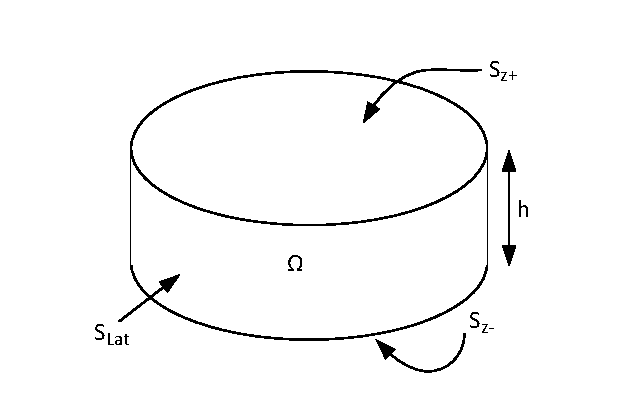
\includegraphics[width=1\linewidth]{figures/problem4_isometric}
		\caption{3D isometric view}
	\end{subfigure}
	\hspace{10mm}
	\begin{subfigure}{.45\textwidth}
		\hspace{0.5cm}
		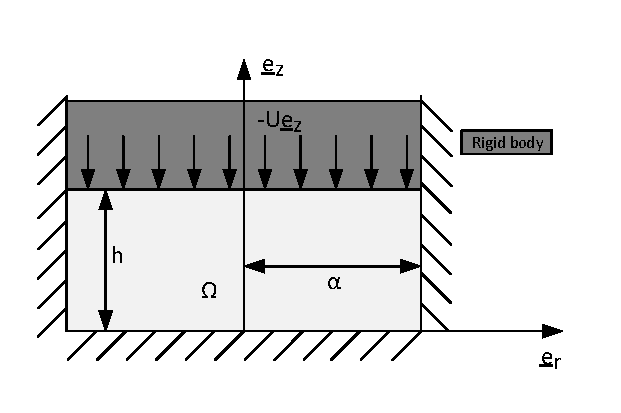
\includegraphics[width=1\linewidth]{figures/problem4_2d}
		\caption{cross-sectional view}
	\end{subfigure}	
	\caption{Oedometric compression}
	\label{fig:problem4}
\end{figure}

\noindent \textbf{Question 1}: Write the complete problem: kinematic + static + constitutive equation! \\

\textbf{Answer:} Kinematic admissibility:

\begin{equation}
\underline{u} \cdot \underline{n} = 0 \quad \forall \Mu \in S_{Lat} \rightarrow u_r = 0 \quad \forall \Mu \in S_{Lat} 
\end{equation}
\begin{equation}
\underline{n} \cdot \underline{u}  = -U \quad \forall \Mu \in S_{z}^+ \rightarrow u_z = -U \quad \forall \Mu \in S_{z}^+ 
\end{equation}
\begin{equation}
\epsuu (\underline{u}) = \frac{1}{2} ({\Graduu \uu + \Graduu^T \uu }) \quad \forall \Mu \in \Omega
\end{equation}
\begin{equation}
\underline{u} \cdot \underline{n} = 0 \quad \forall \Mu \in S_{z}^- \rightarrow u_z = 0 \quad \forall \Mu \in S_{z}^- 
\end{equation} \\

Static admissibility:
\begin{equation}
\divu \sigmauu = \underline{0} \quad \forall \Mu \in \Omega 
\end{equation}
or in expanded form as below
\begin{equation}
\begin{split}
& \sigmarr ,_r + \frac{1}{r} (\sigmart,_\theta + \sigmarr - \sigmatt) + \sigmarz,_z = 0 \\
& \sigmatr ,_r + \frac{1}{r} (\sigmatt,_\theta + \sigmart + \sigmatr) + \sigmatz,_z = 0 \\
& \sigmazr ,_r + \frac{1}{r} (\sigmazt,_\theta + \sigmazr ) + \sigmazz,_z = 0
\end{split} \quad \quad  \rightarrow \quad \quad \forall \Mu \in \Omega 
\end{equation}

Contact without friction:
\begin{equation}
(\sigmauu \cdot \tu)\cdot \tu = 0 \quad \forall \Mu \in S_z^+ \rightarrow \sigmarz = \sigmatz = 0 \quad \Mu \in S_z^+
\label{eq:szplus}
\end{equation}

Contact without friction:
\begin{equation}
(\sigmauu \cdot \tu)\cdot \tu = 0 \quad \forall \Mu \in S_z^- \rightarrow \sigmarz = \sigmatz = 0 \quad \Mu \in S_z^-
\label{eq:szmin}
\end{equation}

Contact without friction:
\begin{equation}
(\sigmauu \cdot \tu)\cdot \tu = 0 \quad \forall \Mu \in S_{Lat} \rightarrow \sigmatr = \sigmatz = 0 \quad \Mu \in S_{Lat}
\label{eq:slat}
\end{equation}

Constitutive equations:
\begin{equation}
\sigmauu = \lambda \text{tr} \epsuu \underline{\underline{1}} + 2 \mu \epsuu \quad \forall \Mu \in \Omega
\end{equation}



\noindent \textbf{Question 2}: Assume that $\uu = - \frac{U}{h} z \eu_z $. Is this kinematically admissible? \\

\textbf{Answer:} We assume that
\begin{equation}
\uu = \left(
\begin{matrix}
0 \\ 0 \\ -\frac{U}{h}z
\end{matrix}
\right) = \left(
-\frac{U}{h}z
\right) \quad \text{Of course } \uu \text{ is kinematically admissible.}
\end{equation}
By definition (using the gradient of a vector with cylindrical coordinates):
\begin{equation}
\Graduu \cdot \uu = \left[
\begin{matrix}
0 &0 &0 \\
0 &0 &0 \\
0 &0 &-\frac{U}{h} \\
\end{matrix}
\right] \rightarrow \epsuu = \left[
\begin{matrix}
0 &0 &0 \\
0 &0 &0 \\
0 &0 & \epszz \\
\end{matrix}
\right]
\end{equation}
with $\epszz = -U/h \rightarrow $ the compatibility equation is obviously satisfied. \\

\noindent \textbf{Question 3}: Find the corresponding stress $\sigmauu$. Is it statistically admissible? \\

\textbf{Answer:} 
\begin{equation}
\sigmauu = \lambda \text{tr} \epsuu \underline{\underline{1}} + 2 \mu \epsuu \rightarrow \sigmauu = \left[
\begin{matrix}
-\lambda \frac{U}{h} &0 &0 \\
0 &-\lambda \frac{U}{h} &0 \\
0 &0 & -(\lambda+2\mu) \frac{U}{h} \\
\end{matrix}
\right]
\end{equation} 
Eqs. \ref{eq:slat}, \ref{eq:szmin}, and \ref{eq:szplus} are obviously satisfied.
$\divu \sigmauu \rightarrow$ obviously equal to 0 as $\sigmauu $ is constant. \\

\noindent \textbf{Question 4}: Find oedometric  modulus $\hat{E}$ as a  function of $E$ and $\nu$.

\textbf{Answer:} The vertical force is equal to 
\begin{equation}
\Pu = \int_{S_z^+} \sigmauu \cdot \eu_z dS_3^+
\end{equation}
\begin{equation}
\Pu = \int_{S_z^+} - (\lambda + 2\mu)\frac{U}{h} dS_3^+ \eu_z = -\Pu \eu_z \quad \text{with} \quad \Pu = \frac{(\lambda+2\mu)US}{h} 
\end{equation}
So we can identify the oedometric modulus $\hat{E} = \lambda + 2\mu$.

\begin{equation}
\begin{split}
 \sigmauu &= \lambda \text{tr} \epsuu \underline{\underline{1}} + 2 \mu \epsuu \\
 \epsuu &= \frac{1+\nu}{E} \sigmauu - \frac{\nu}{E} \text{tr} \sigmauu \underline{\underline{1}}
\end{split} \quad \rightarrow \quad  
\begin{split}
\text{tr} \sigmauu &= (3\lambda + 2\mu) \text{  tr} \epsuu \\
\text{tr} \epsuu &= (\frac{1-2\nu}{E}) \text{  tr} \sigmauu \\
\end{split} \quad \rightarrow \quad 3\lambda + 2\mu = \frac{E}{1-2\nu}
\end{equation}

Or we can also write as follows:
\begin{equation}
\text{tr} \sigmauu = (3\lambda + 2\mu) \text{tr} \epsuu \quad \rightarrow \quad \sigmauu = \frac{\lambda}{3\lambda + 2\mu} \text{tr} \sigmauu \underline{\underline{1}} + 2\mu \epsuu
\end{equation}
\begin{equation}
\epsuu = \frac{1}{2\mu} \sigmauu - \frac{\lambda}{2\mu (3\lambda + 2\mu)} \text{tr} \sigmauu \underline{\underline{1}}
\end{equation}

By identification, 
\begin{equation}
\frac{1}{2\mu} = \frac{1+\nu}{E} \quad  \text{     and     } \quad \frac{\lambda}{2\mu (3\lambda + 2\mu)} = \frac{\nu}{E}  
\end{equation}
\begin{equation}
\rightarrow \lambda = \frac{E \nu}{(1+\nu)(1-2\nu)} \quad  \text{     and     } \quad \mu = \frac{E}{2(1+\nu)}
\end{equation}
Thus, 
\begin{equation}
\hat{E} = \lambda + 2\mu = \frac{2 E\nu + 2E(1-2\nu)}{2(1+\nu)(1-2\nu)} = \frac{E(1-\nu)}{(1+\nu)(1-2\nu)}
\end{equation}



\end{document}